\iffalse
\begin{frame}{Champ de repère non-orthogonal}
    \centering
    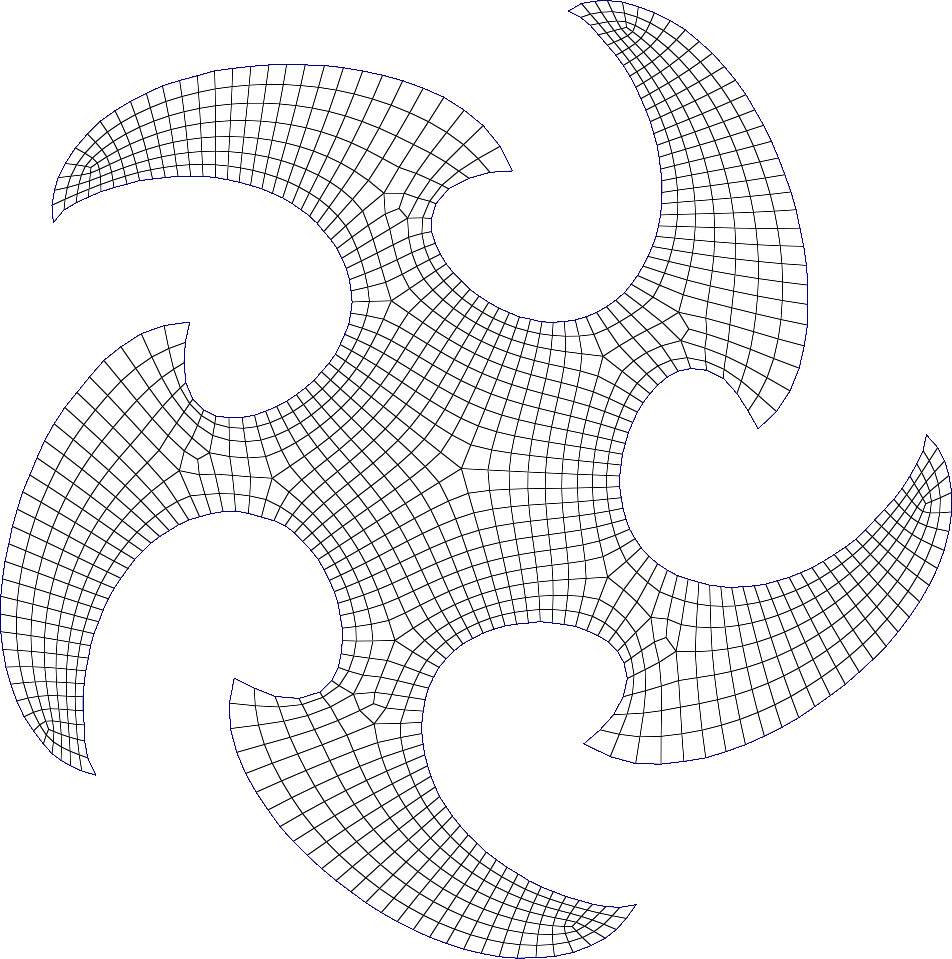
\includegraphics[width=0.4\linewidth]{img_spm_ff/shuriken_big_quads.PNG}
    \includegraphics[width=0.4\linewidth]{img_spm_ff/shuriken_nonortho.png}

\end{frame}
\fi

\begin{frame}{Motivations : Maillage quadrilatère}
    \centering
    
    \begin{minipage}[c]{0.48\textwidth}
    \centering 
    \textbf{Champ orthogonal}\\
    \vspace{0.3cm}
    \begin{adjustbox}{width=0.8\linewidth,clip,trim=0 0 {.48\width} 0}
        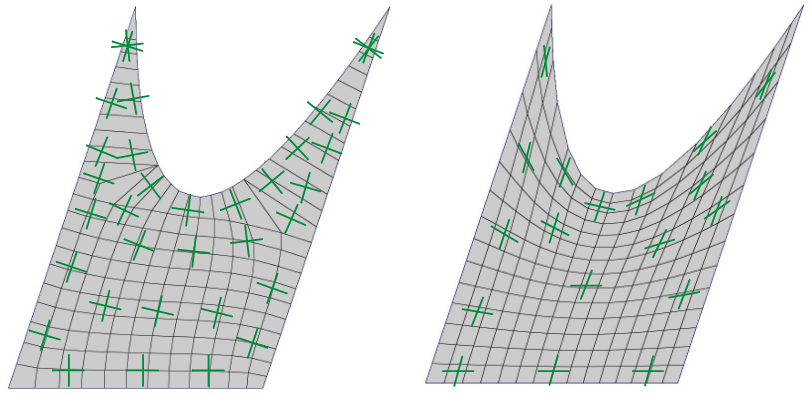
\includegraphics{img_spm_ff/comp1.png}
    \end{adjustbox}
    \end{minipage}%
    \hfill\vline\hfill
    \begin{minipage}[c]{0.48\textwidth}
    \centering 
    \textbf{Champ non-orthogonal}\\
    \vspace{0.3cm}
    \begin{adjustbox}{width=0.75\linewidth,clip,trim={.52\width} 0 0 0}
        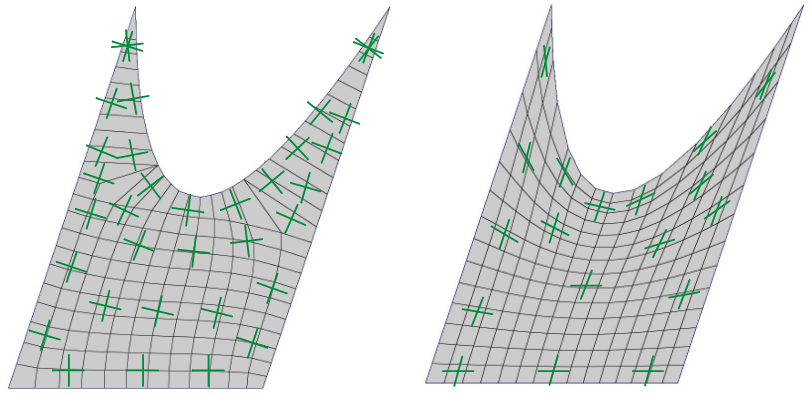
\includegraphics{img_spm_ff/comp1.png}
    \end{adjustbox}
    \end{minipage}
    
    \vspace*{0.3cm}
    \begin{itemize}
         \item Un champ 2D orthogonal ne gère pas les coins de petit angle.
         \item Ce travail permet l'optimisation de repères 2D non-orthogonaux.
    \end{itemize}
    
\end{frame}

\begin{frame}{Qu'est-ce qui est difficile ?}
    \centering
    %To compare two 2D frames, we can't directly compare their vectors $(\vec{u}, \vec{v})$, as a same frame is given by many different combinations of vectors : 
    \small
    \begin{itemize}
     \item Un repère est défini comme un ensemble de vecteurs : $$\mathcal{U} = \left\{\vec{u},\ -\vec{u},\ \vec{v},\ -\vec{v}\right\}$$ 
     \item Comment minimiser la "distance" entre les repères voisins d'un champ ?
     
     %\item Distance definition between 2 sets $\mathcal{U}_i$ and $\mathcal{U}_j$ ?
     %\item Using distance of vectors induces finding a matching between sets \\%If you want to compare sets by comparing their vectors, you need to match each vector\\
   \end{itemize}
      \vspace*{0.5\baselineskip}
      
    \begin{overprint}
    \onslide<1> \centering
    
\includegraphics[width=0.6\linewidth]{img_spm_ff/dist_question.PNG}
      %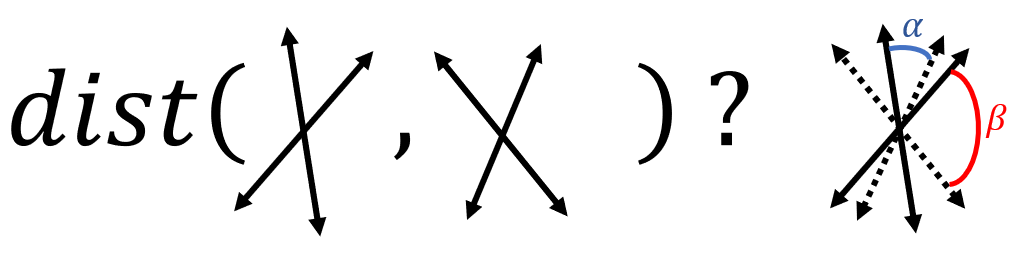
\includegraphics[width=0.8\linewidth]{vector_dist_1.PNG}
      %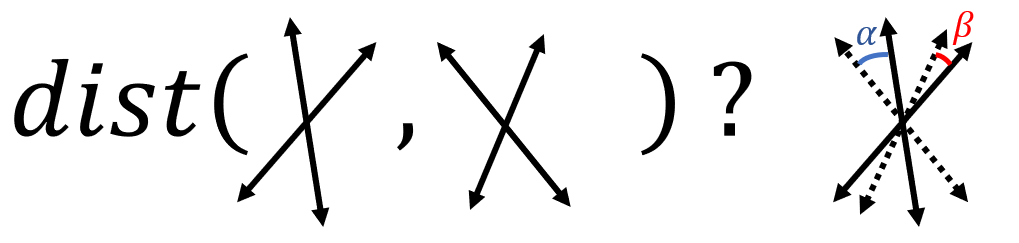
\includegraphics[width=0.8\linewidth]{vector_dist_2.PNG}
    \onslide<2> 
            \centering
      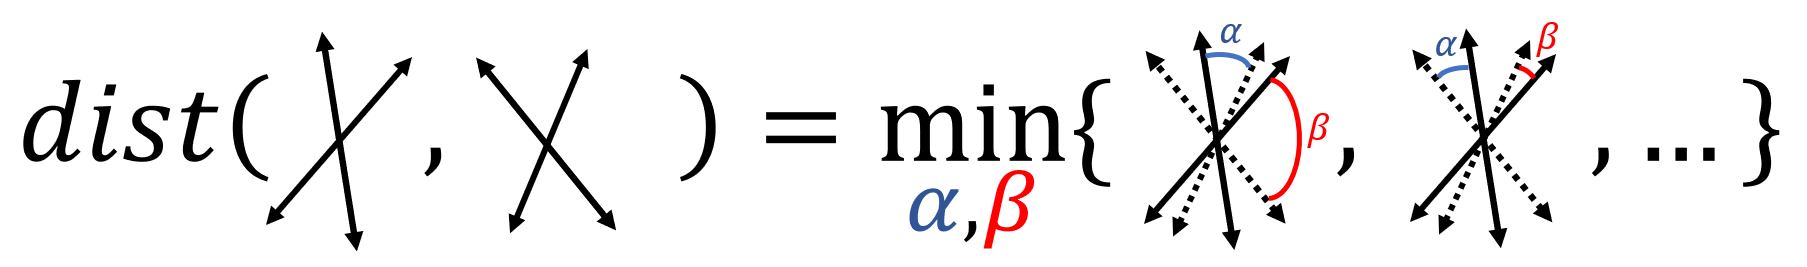
\includegraphics[width=\linewidth]{img_spm_ff/dist_sol.PNG}
        
        Problème : Cette définition de distance est trop difficile à minimiser globalement de part sa nature combinatoire (choix de correspondance).
    
    \end{overprint}
    \normalsize
\end{frame}


\begin{frame}{Repère 2D en tant que fonction polynomiale}
    \centering
    
$\mathcal{U} = \left\{\vec{u},\ -\vec{u},\ \vec{v},\ -\vec{v}\right\}$  est représenté par un polynôme \\
\textbf{restreint au cercle unité}
$$P_\mathcal{U}(\vec{s}) = \langle \vec{u},\ \vec{s}\rangle^{4} +  \langle \vec{v},\ \vec{s}\rangle^{4}, \ \ \   \forall \vec{s} \in {\rm I\!R}^2, \lVert \vec{s} \rVert = 1$$

     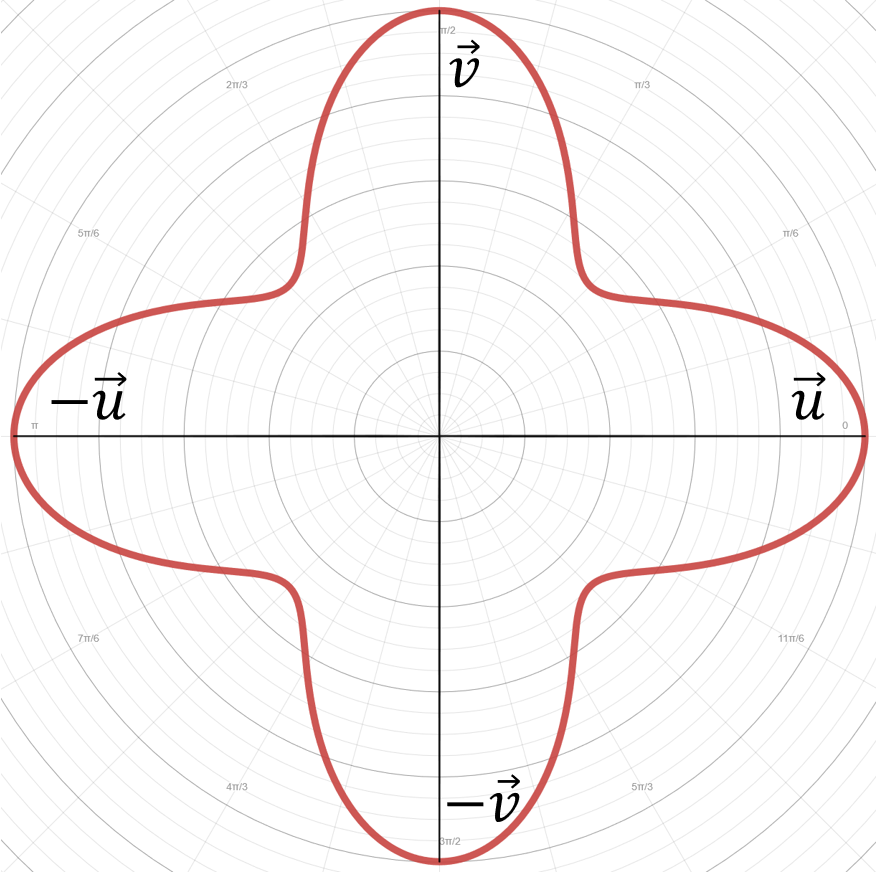
\includegraphics[width=0.3\linewidth]{img_spm_ff/anoted_orthogonal.PNG}
    \ \ \ 
       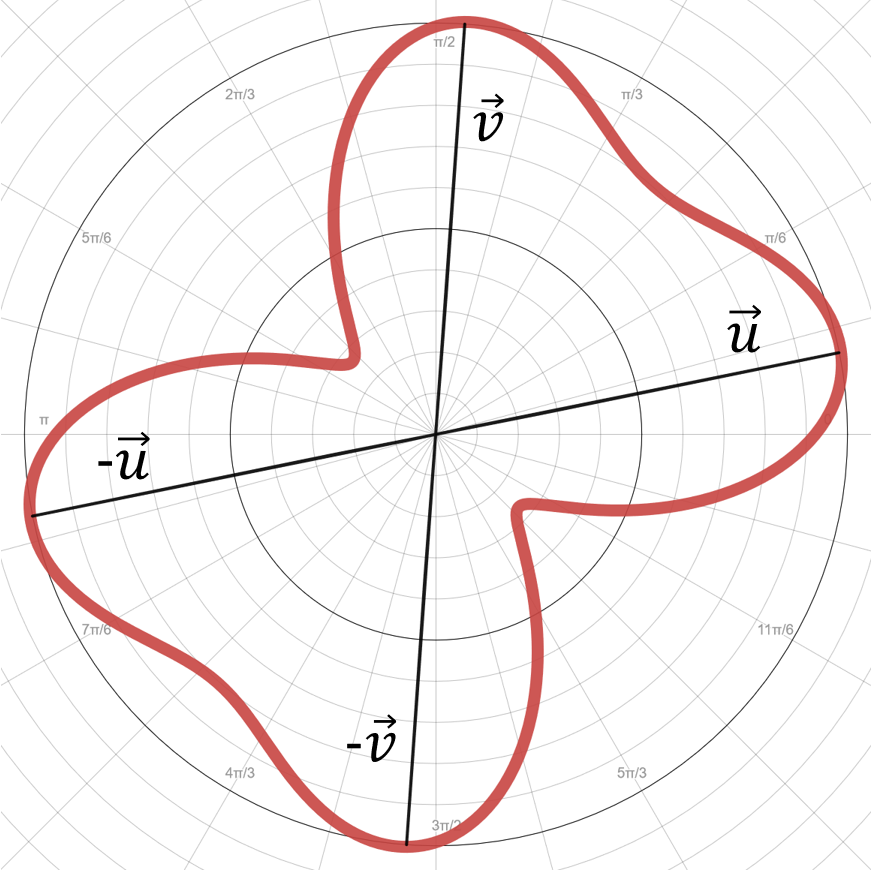
\includegraphics[width=0.3\linewidth]{img_spm_ff/anoted_polynome.PNG}
    \\
    
    \normalsize
    \begin{itemize}
    %\item $P_\mathcal{U}(\vec{s}) = \langle \vec{u},\ \vec{s}\rangle^{4} +  \langle \vec{v},\ \vec{s}\rangle^{4}, \ \ \   \forall \vec{s} \in {\rm I\!R}^2, \lVert \vec{s} \rVert = 1$
     \item $dist(\mathcal{U}_i, \mathcal{U}_j) = \int (P_{\mathcal{U}_i} - P_{\mathcal{U}_j})^2$
    \end{itemize}
\end{frame}

\begin{frame}{Décomposition dans la base de Fourier}
    \centering
    \begin{overprint}
    \onslide<2> \centering
    Avec $v = u^{\perp}$, même représentation que [\cite{palacios_rotational_2007}].
    
    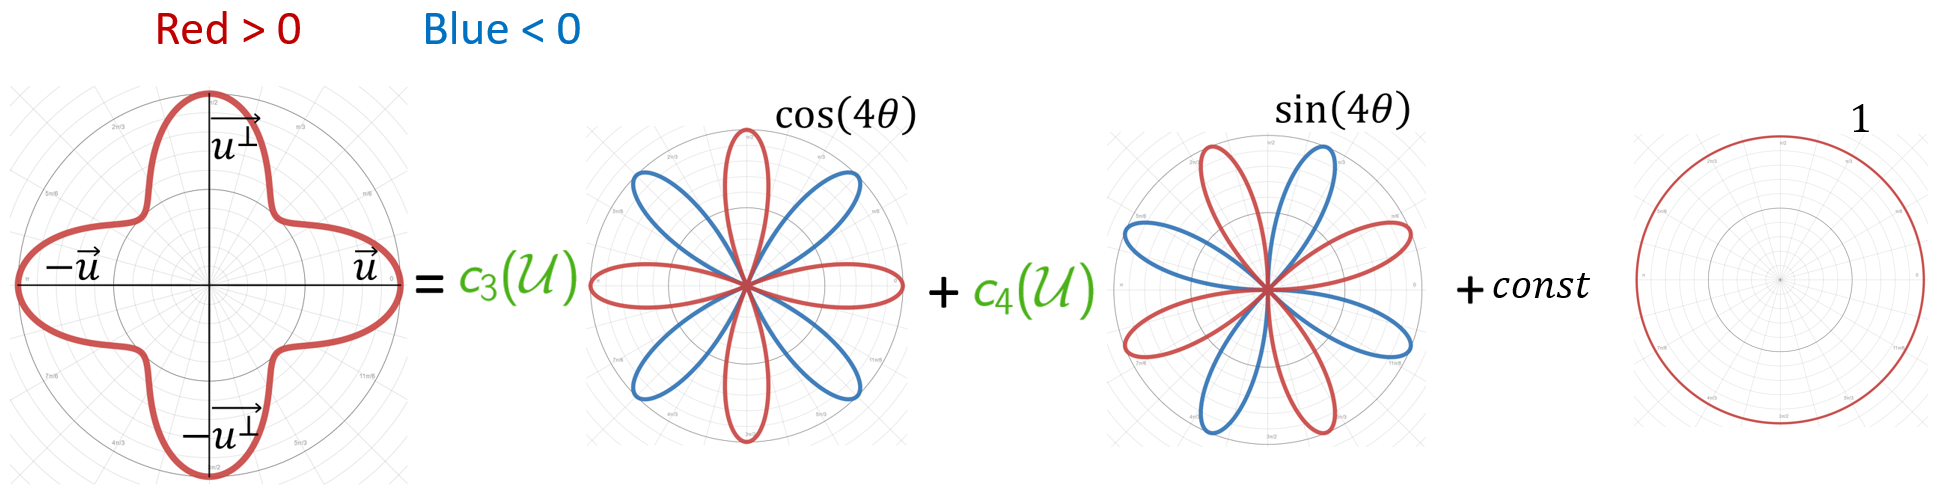
\includegraphics[width=0.95\linewidth]{img_spm_ff/ortho_decomposition_with_circle.PNG}
    
    $$ dist(\mathcal{U}_i, \mathcal{U}_j) =  \int (P_{\mathcal{U}_i} - P_{\mathcal{U}_j})^2 =  \left({\color{green}c_3(\mathcal{U}_i)} - {\color{green}c_3(\mathcal{U}_j)} \right)^2 
    + \left({\color{green}c_4(\mathcal{U}_i)} - {\color{green}c_4(\mathcal{U}_j)} \right)^2$$
    \onslide<1> \centering
    
    Décomposer $P_\mathcal{U}$ dans la base de Fourier simplifie $dist(\mathcal{U}_i, \mathcal{U}_j)$. \\
    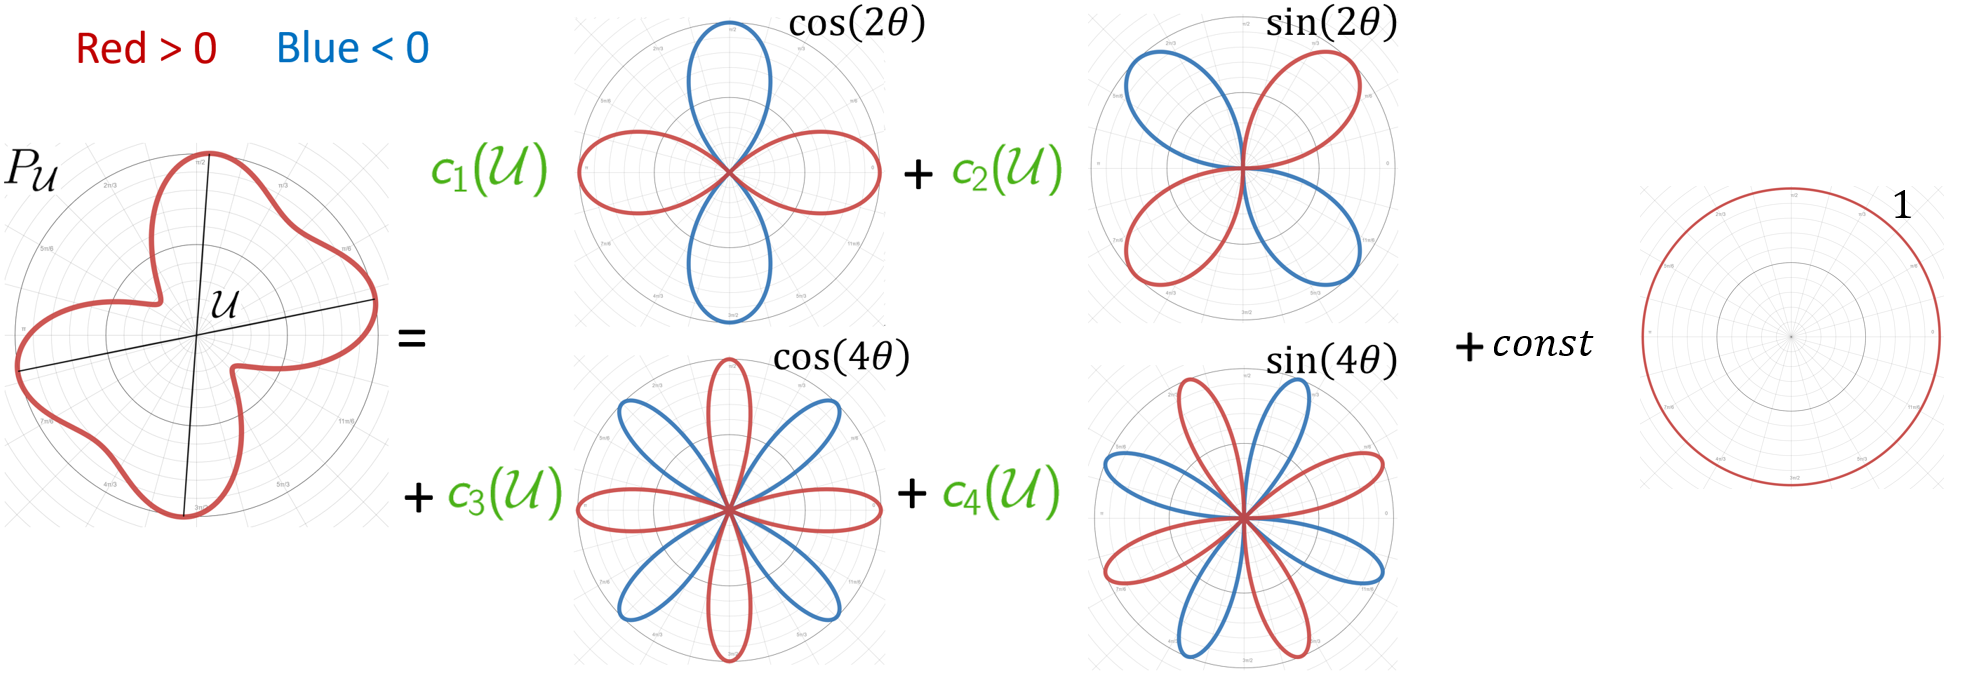
\includegraphics[width=0.95\linewidth]{img_spm_ff/polynome_decomposition_with_circle.PNG}
    $$ dist(\mathcal{U}_i, \mathcal{U}_j) =  \int (P_{\mathcal{U}_i} - P_{\mathcal{U}_j})^2 = \sum_{\ell=1}^4 \left({\color{green}c_\ell(\mathcal{U}_i)} - {\color{green}c_\ell(\mathcal{U}_j)} \right)^2$$
    \end{overprint}
    
\end{frame} 

\begin{frame}{Optimisation d'un champ non-orthogonal 2D}
    \centering
    \small
    %From the decomposition in the Fourier basis, we define
    %$$ dist(\mathcal{U}_i, \mathcal{U}_j) =  \int (P_{\mathcal{U}_i} - P_{\mathcal{U}_j})^2 = \sum_{\ell=1}^4 \left({\color{green}c_\ell(\mathcal{U}_i)} - {\color{green}c_\ell(\mathcal{U}_j)} \right)^2$$
    Pour calculer un champ de repère non-orthogonal 2D lisse, minimiser :
    $$ E_{tot} = \sum_{Voisins(i, j)} dist(\mathcal{U}_i, \mathcal{U}_j)$$
    
    Contrôle de l'orthogonalité: $c_1, c_2, c_3, c_4 \mapsto \lambda c_1, \lambda c_2, c_3, c_4$ 
     
     \vspace*{0.5\baselineskip}
     %modifies the orthogonality of the field : 
    \begin{minipage}[b]{0.15\textwidth}
        \centering
        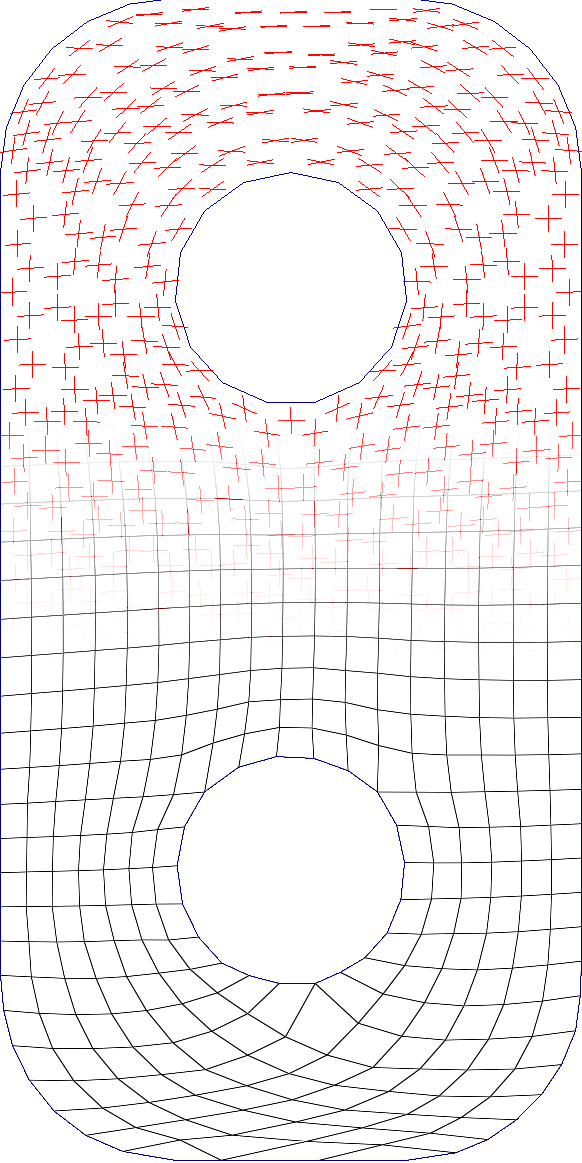
\includegraphics[width=\textwidth]{img_spm_ff/perced_1}
        $\lambda = 0.1$
    \end{minipage}
    \ \ \ 
    %\hfill
    \begin{minipage}[b]{0.15\textwidth}
        \centering
        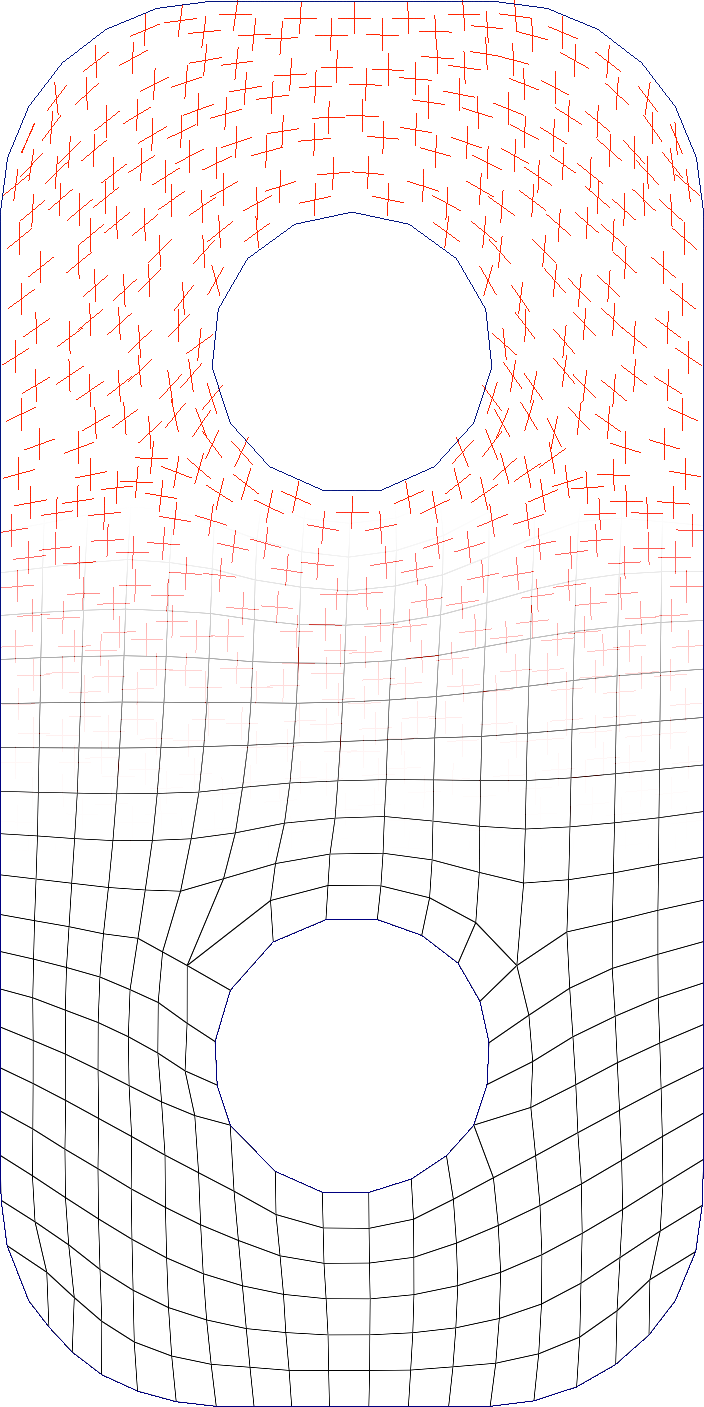
\includegraphics[width=\textwidth]{img_spm_ff/perced_9}
        $\lambda = 0.5$
    \end{minipage}
    %\hfill
    \ \ \ 
    \begin{minipage}[b]{0.15\textwidth}
        \centering
        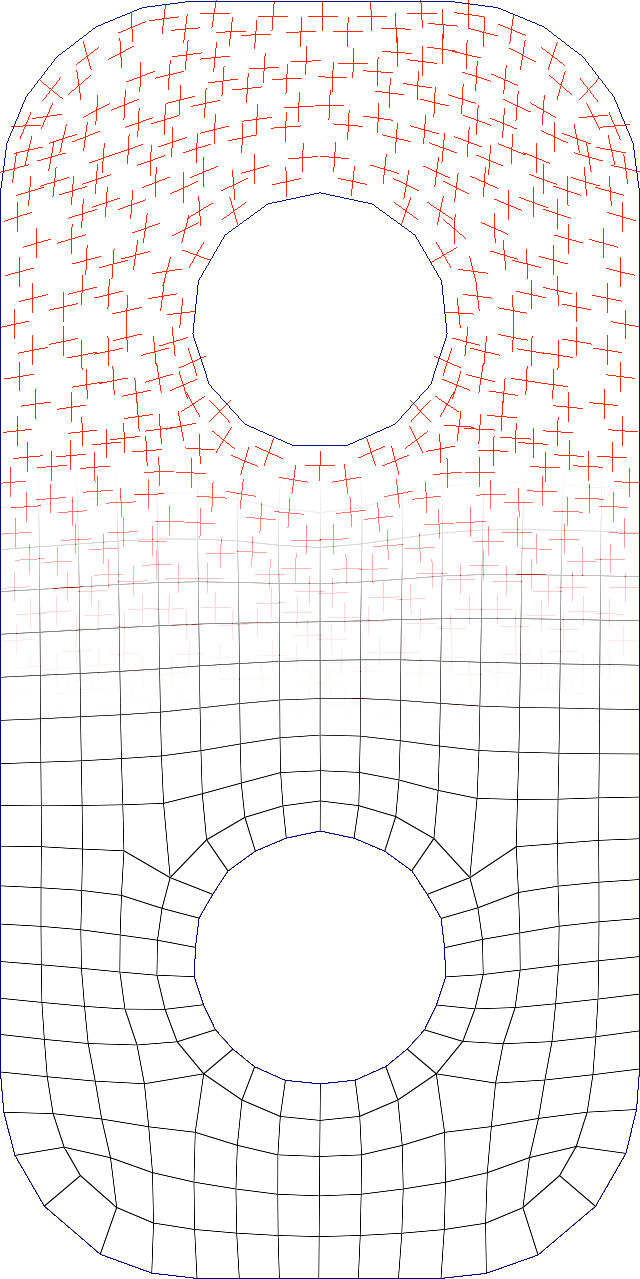
\includegraphics[width=\textwidth]{img_spm_ff/perced_16}
        $\lambda = 1$
    \end{minipage}
    %\hfill
    \ \ \ 
    \begin{minipage}[b]{0.15\textwidth}
        \centering
        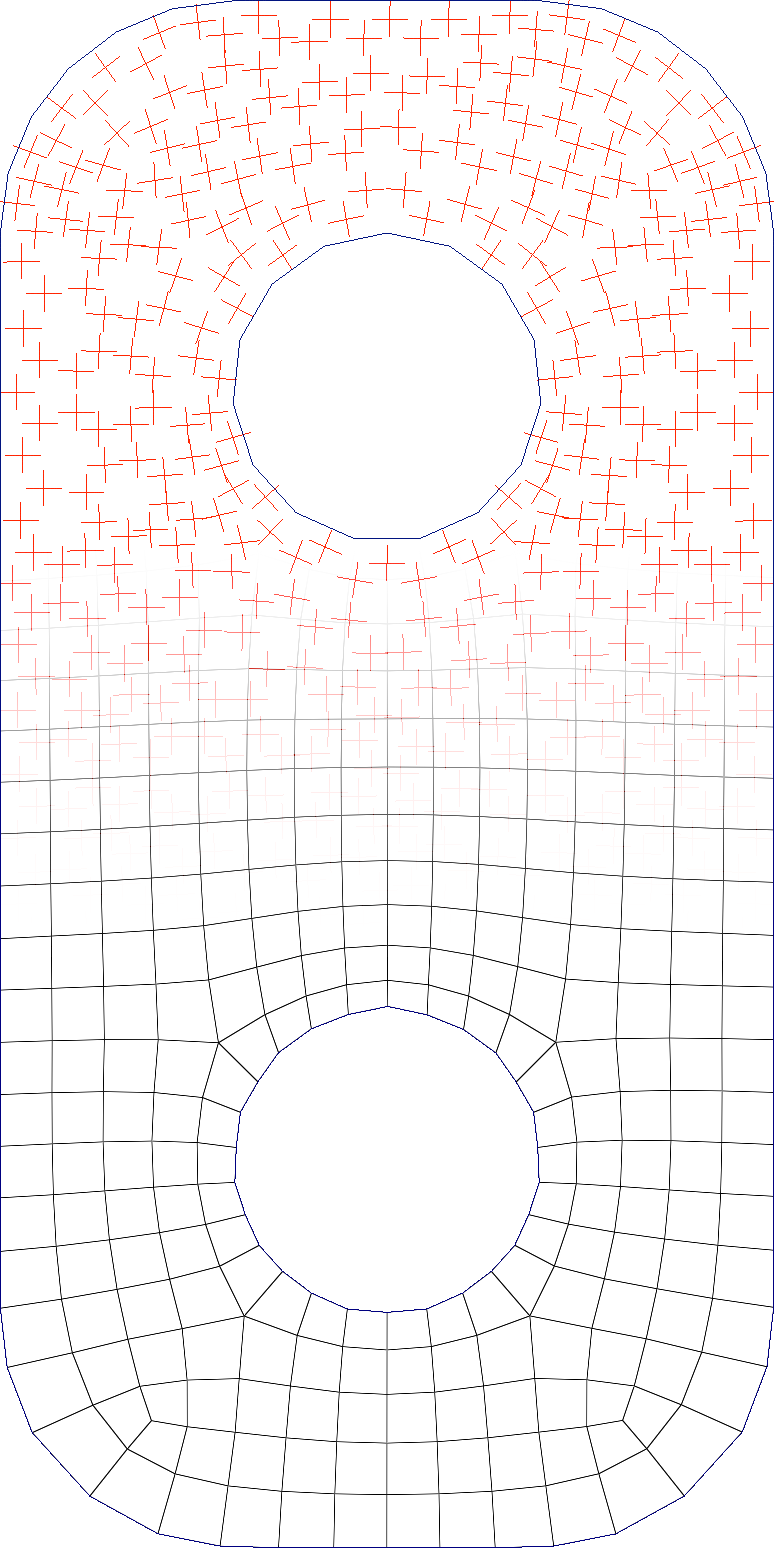
\includegraphics[width=\textwidth]{img_spm_ff/perced_25}
        $\lambda = 1.5$
    \end{minipage}
\end{frame} 

\begin{frame}{Maillages obtenus avec des champs non-orthogonaux}
    \centering
    \includegraphics[width=.49\textwidth]{img/spmff/shuriken_nonortho}
    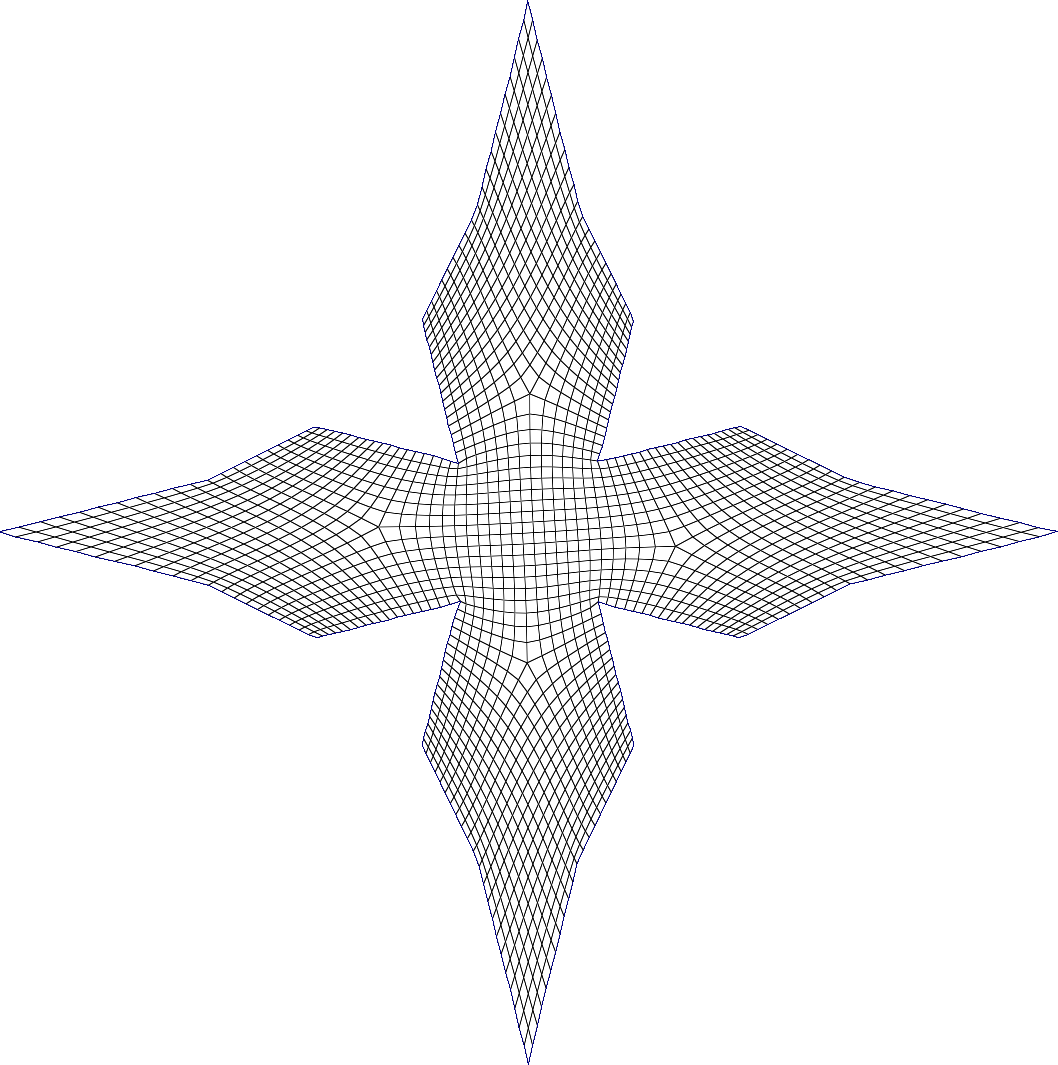
\includegraphics[width=.49\textwidth]{img/spmff/shuriken_center_singu}
    %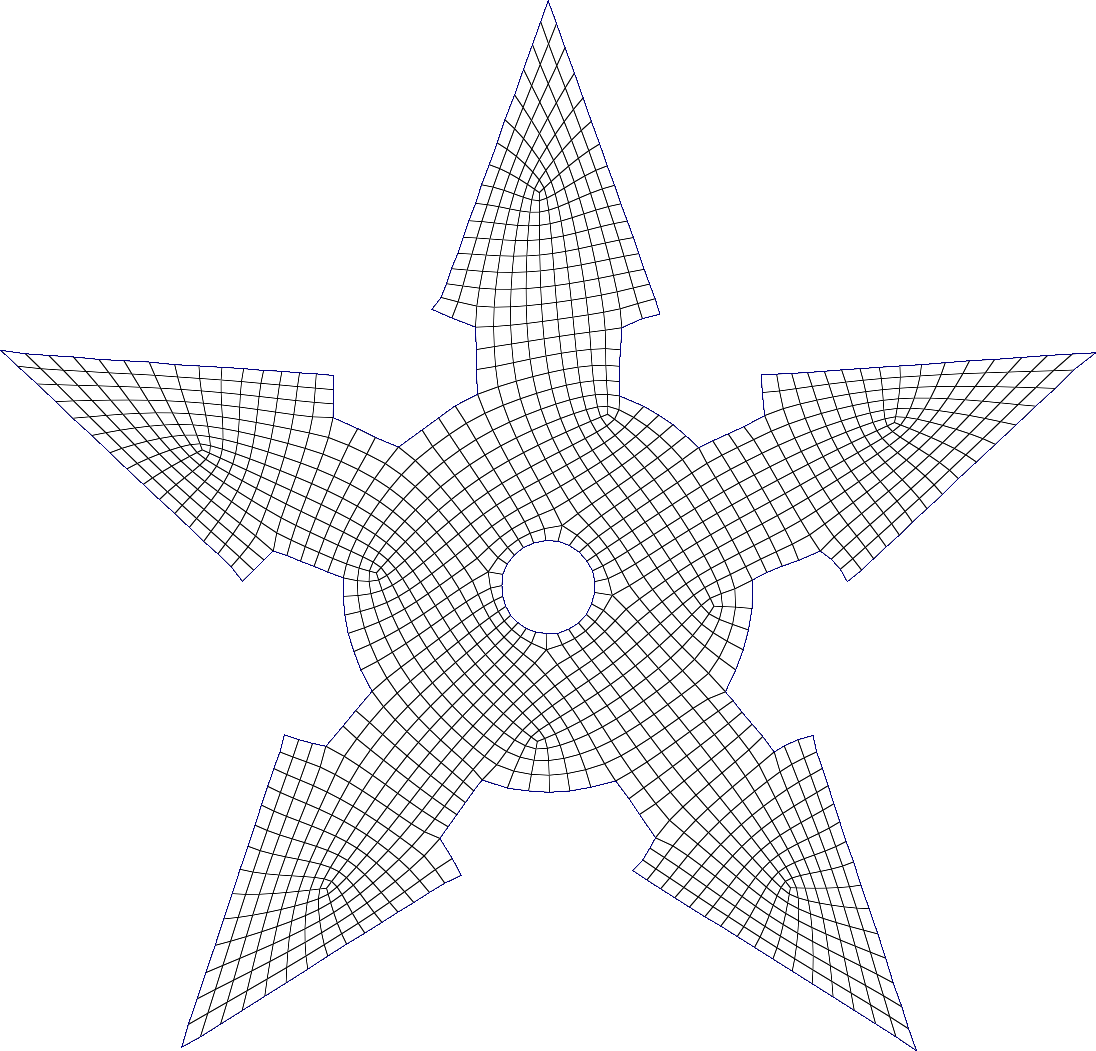
\includegraphics[width=.49\textwidth]{img/spmff/shuriken_fleches}
    %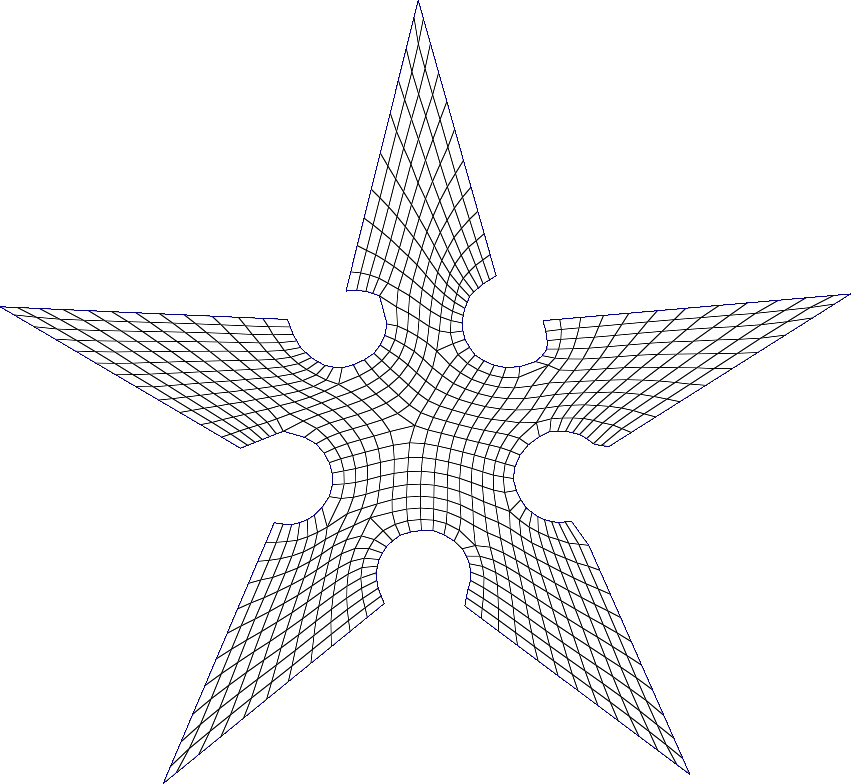
\includegraphics[width=.49\textwidth]{img/spmff/quads_nonortho_shurik0}
    %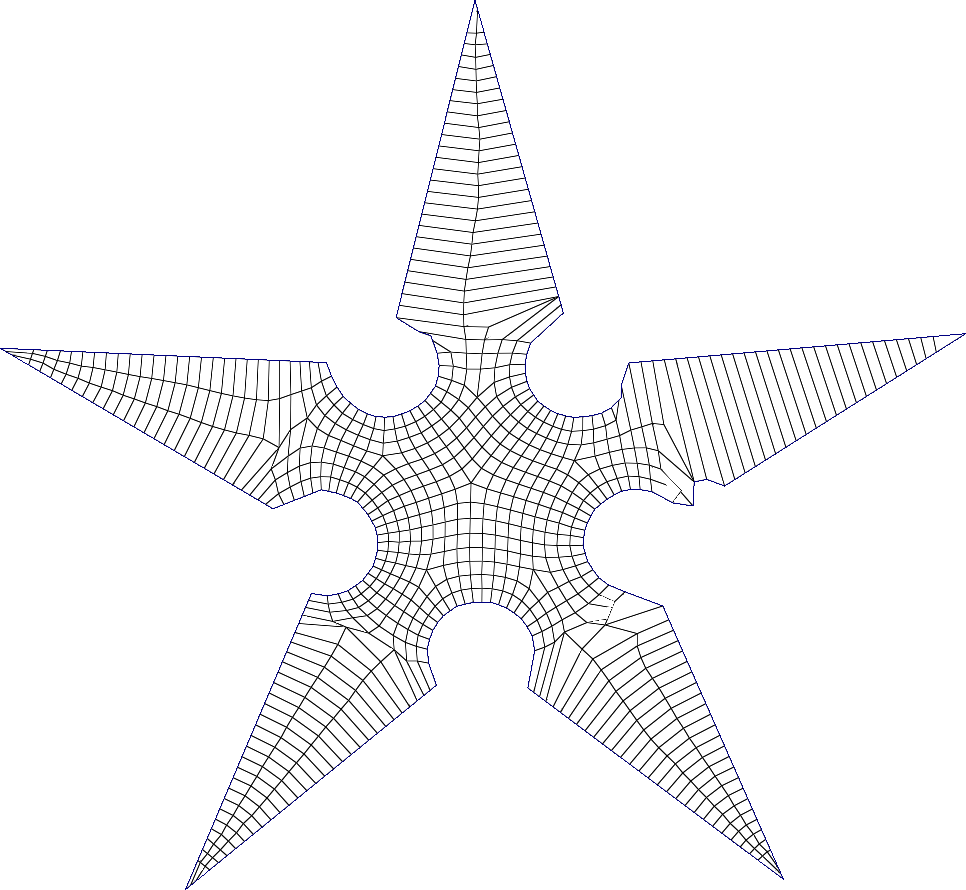
\includegraphics[width=.49\textwidth]{img/spmff/quads_ortho_shurik0}
    %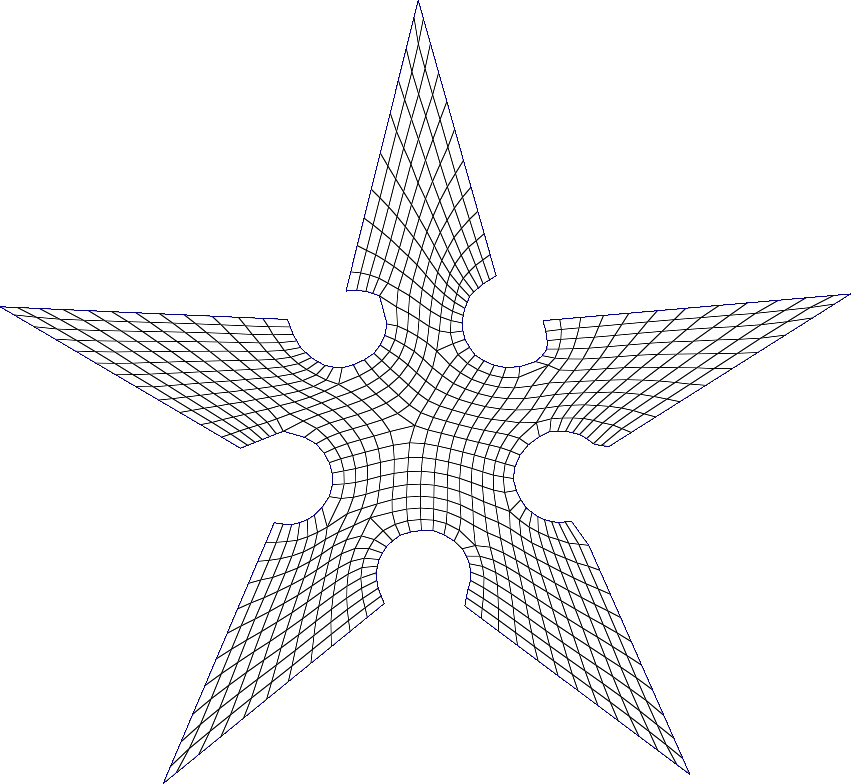
\includegraphics[width=.49\textwidth]{img/spmff/quads_nonortho_shurik0}
\end{frame}
